\titledquestion{Maximum area rectangle in histogram}

We are given a histogram consisting of $n$ parallel bars side by side, each of width $1$, as well as a sequence $A$ containing the heights of the bars where the height of the $i$th bar is $\mathbf{a}_i$ for $\forall \; i \in [n]$. For example, the figures below show the case where $n= 7$ and $A = \langle 6, 2, 5, 4, 4, 1, 3 \rangle$. Our goal is to find the maximum area of the rectangle placed inside the boundary of the given histogram with a \textbf{divide-and-conquer} algorithm. (Here you don't need to find which rectangle maximizes its area.)

Reminder: There do exist algorithms that solve this problem in linear time. However, you are \textbf{not allowed} to use them in this homework. Any other type of algorithms except the divide-and-conquer ones will get \textbf{no} credit.

\begin{figure}[htbp]
    \centering
    \begin{minipage}[t]{0.48\textwidth}
        \centering
        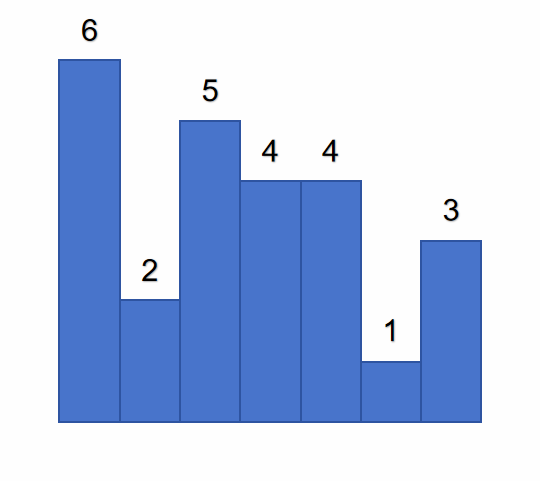
\includegraphics[width=6cm]{withnum.png}
        \caption{The Original Histogram}
    \end{minipage}
    \begin{minipage}[t]{0.48\textwidth}
        \centering
        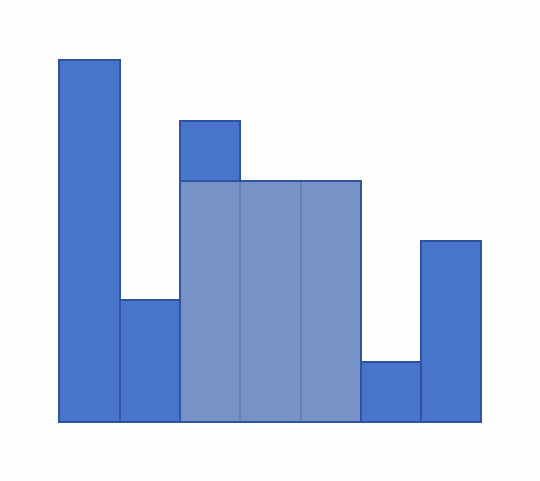
\includegraphics[width=6cm]{withrect.png}
        \caption{The Largest Rectangle in Histogram}
    \end{minipage}
\end{figure}

You may use $Rect(l, r, A)$ to represent the answer of the sub-problem w.r.t. the range $\left[l, r\right]$.

\begin{parts}
    \part[3] \textbf{Briefly} describe:
    \begin{enumerate}
        \item How would you divide the original problem into 2 sub-problems?
        \item Under what circumstances will the answer to the original problem not be covered by the answers of the 2 sub-problems?
        \item Given the answers of the 2 sub-problems, how would you get the answer of the original problem?
    \end{enumerate}

    \begin{solution}
        %%%%%%%%%%%%%%%%%%%%%%%%%%%%%%%%%%%%%%%%%%%%%%%%%
        % Replace `\vspace{2in}' with your answer.
        \begin{enumerate}
            \item
                  Identify the middle bar of the histogram. This bar will be part of the maximum area rectangle or the rectangle will be entirely to the left or right of it.
                  Split the problem into two sub-problems:
                  \begin{enumerate}
                      \item
                            The maximum area rectangle of the left sub-histogram, consisting of bars to the left of the middle bar.
                      \item
                            The maximum area rectangle of the right sub-histogram, consisting of bars to the right of the middle bar.
                  \end{enumerate}
            \item
                  If the maximum area rectangle is crossing the left and right sub-histogram, then the answer to the original problem will not be covered by the answers of the 2 sub-problems.
            \item
                  First caculate the maximum area rectangle consisting the middle bar.
                  Then compare the maximum area rectangle among the 2 sub-problems' answers and the caculated area.
                  The maximum area rectangle among the 3 areas is the answer of the original problem.
        \end{enumerate}
        %%%%%%%%%%%%%%%%%%%%%%%%%%%%%%%%%%%%%%%%%%%%%%%%%
    \end{solution}

    \part[8] Based on your idea in part(a), design a \textbf{divide-and-conquer} algorithm for this problem. Make sure to provide \textbf{clear description} of your algorithm design in \textbf{natural language}, with \textbf{pseudocode} if necessary.

    \begin{solution}
        %%%%%%%%%%%%%%%%%%%%%%%%%%%%%%%%%%%%%%%%%%%%%%%%%
        % Replace `\vspace{7.5in}' with your answer.
        \begin{enumerate}
            \item If $l > r$, return 0 (base case with no bars in the range).
            \item Identify the middle bar index as $m = \frac{l + r}{2}$.
            \item Left maximum area rectangle: $\text{Rect}(l, m - 1, A)$
            \item Right maximum area rectangle: $\text{Rect}(m + 1, r, A)$
            \item Calculate the maximum area rectangle that includes the middle bar:
                  \begin{enumerate}
                      \item Initialize variables: $\text{min\_height} = A[m]$ (minimum height is the height of the middle bar)
                      \item Initialize $\text{area} = \text{min\_height}$
                      \item Iterate from the middle bar towards the left ($i = m - 1$) and towards the right ($i = m + 1$):
                            \begin{enumerate}
                                \item Update $\text{min\_height}$ as $\min(\text{min\_height}, A[i])$
                                \item Calculate $\text{area}$ as $\max(\text{area}, \text{min\_height} \times (j - l + 1))$ where $j$ is the current index
                            \end{enumerate}
                  \end{enumerate}


            \item
                  Return the maximum of Left, Right, and the area calculated in step 5.
        \end{enumerate}

        %%%%%%%%%%%%%%%%%%%%%%%%%%%%%%%%%%%%%%%%%%%%%%%%%
    \end{solution}

    \part[2] Provide the run-time complexity analysis of your algorithm in part (b). Make sure to include the \textbf{recurrence relation} of the run-time in your solution.

    \begin{solution}
        %%%%%%%%%%%%%%%%%%%%%%%%%%%%%%%%%%%%%%%%%%%%%%%%%
        % Replace `\vspace{3in}' with your answer.


        The recurrence relation for the algorithm can be expressed as:
        \[
            T(n) = 2T\left(\frac{n}{2}\right) + O(n)
        \]
        where \(n\) is the size of the input array.

        \bigskip

        The Master Theorem gives the solution as \(T(n) = O(n \log n)\).

        \bigskip

        Therefore, the overall runtime complexity of the algorithm is \(O(n \log n)\).

        %%%%%%%%%%%%%%%%%%%%%%%%%%%%%%%%%%%%%%%%%%%%%%%%%
    \end{solution}

\end{parts}